\documentclass[table,dvipsnames]{beamer}
\mode<presentation>{
	\usetheme{Madrid}
	\setbeamercolor{title}{fg=Black,bg=Blue!15}
	\setbeamercolor{frametitle}{fg=Black,bg=Blue!15}
	\setbeamercolor{block title}{fg=Black,bg=Blue!15}
	\setbeamercolor{block}{fg=Black,bg=Blue!10}
}

\usepackage{graphicx}
\usepackage{booktabs}
\usepackage{xcolor}
\usepackage{multirow}
\usepackage{minted}
\usepackage[
type={CC},
modifier={by-sa},
version={4.0},
]{doclicense}

\definecolor{LightGray}{gray}{0.9}

\title[Xirca042022]{Activity Report: Xirca April 2022}
\author{}
\institute[VibrasticLab : \ccbysa]{
	Achmadi ST MT
}
\date{}

\begin{document}
    \begin{frame}
        \titlepage
    \end{frame}

	\section{Tempat dan Jadwal}
	\begin{frame}
		\begin{exampleblock}{Tempat dan Jadwal}
			Kegiatan berlangsung di:
			\begin{itemize}
				\item Tanggal: 18 April 2022 hingga 22 April 2022
				\item Pukul: 08:00 WIB hingga 16:00 WIB
				\item Tempat: Gedung Research and Development PT. Xirca Dama Persada Lantai 2.\\
				Kompleks Puri Syailendra.\\
				Jl. Lemah Neundeut No. Kav-30, Sukawarna, Setrasari, Kota Bandung, Jawa Barat 40164 .
			\end{itemize}
		\end{exampleblock}
	\end{frame}
	
	\section{Kelompok Pekerjaan}
	\begin{frame}
	    \begin{exampleblock}{Kelompok Pekerjaan}
			Lingkup utama pekerjaan yang dilakukan meliputi:
			\begin{itemize}
				\item Assembly 1 unit PCB untuk desain Audiometri P2.
				\item Review Sinyal dan Tone-Generation dari Class-D Audio DAC MAX98357A.
				\item Review sementara desain Audiometri P3.
				\item Upgrade unit packaging untuk Audiometri P2.
			\end{itemize}
	    \end{exampleblock}
	\end{frame}
	
	\section{Assembly PCB}
	\begin{frame}
		\subsection{Tujuan}
		\begin{exampleblock}{Assembly PCB}
			Merakit 1 unit tambahan PCB untuk desain Audiometri P2.
		\end{exampleblock}
	
		\subsection{Hasil}
		\begin{exampleblock}{Assembly PCB}
			Unit tambahan telah terakit
			\begin{center}
				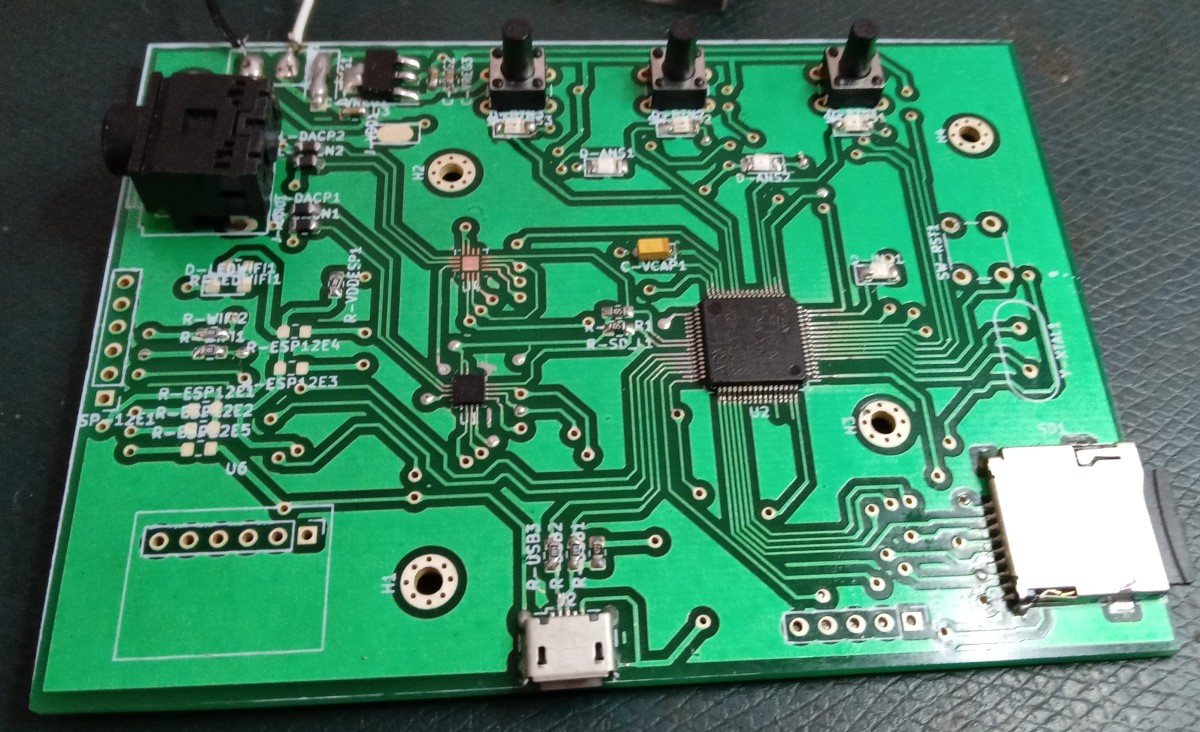
\includegraphics[width=200pt]{images/assembly_hasil}
			\end{center}
		\end{exampleblock}
	\end{frame}

	
	\begin{frame}
		\subsection{Dokumentasi}
		\begin{exampleblock}{Memulai Assembly}
			\begin{center}
				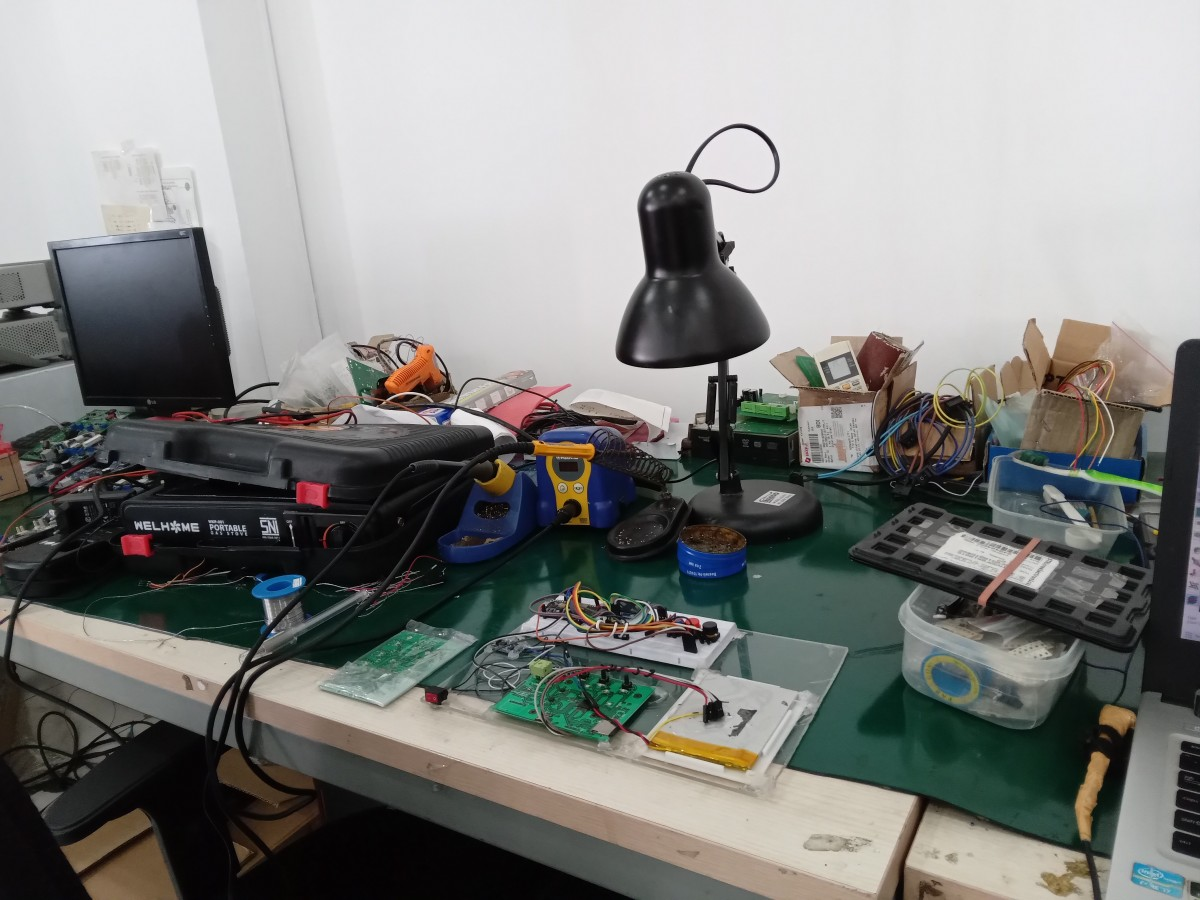
\includegraphics[width=150pt]{images/assembly_unpack}
				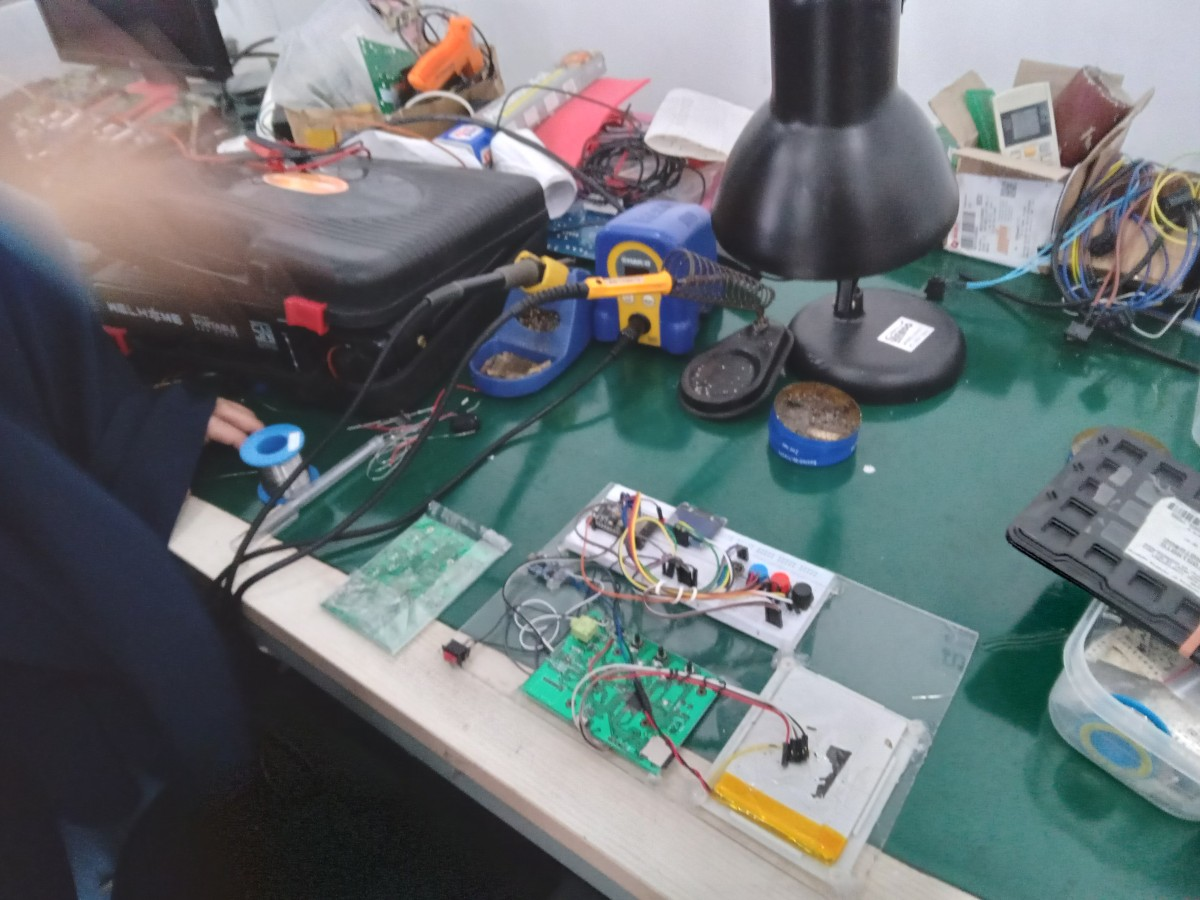
\includegraphics[width=150pt]{images/assembly_start}
			\end{center}
		\end{exampleblock}
	\end{frame}

	\begin{frame}
		\begin{exampleblock}{Proses Soldering Manual}
			\begin{center}
				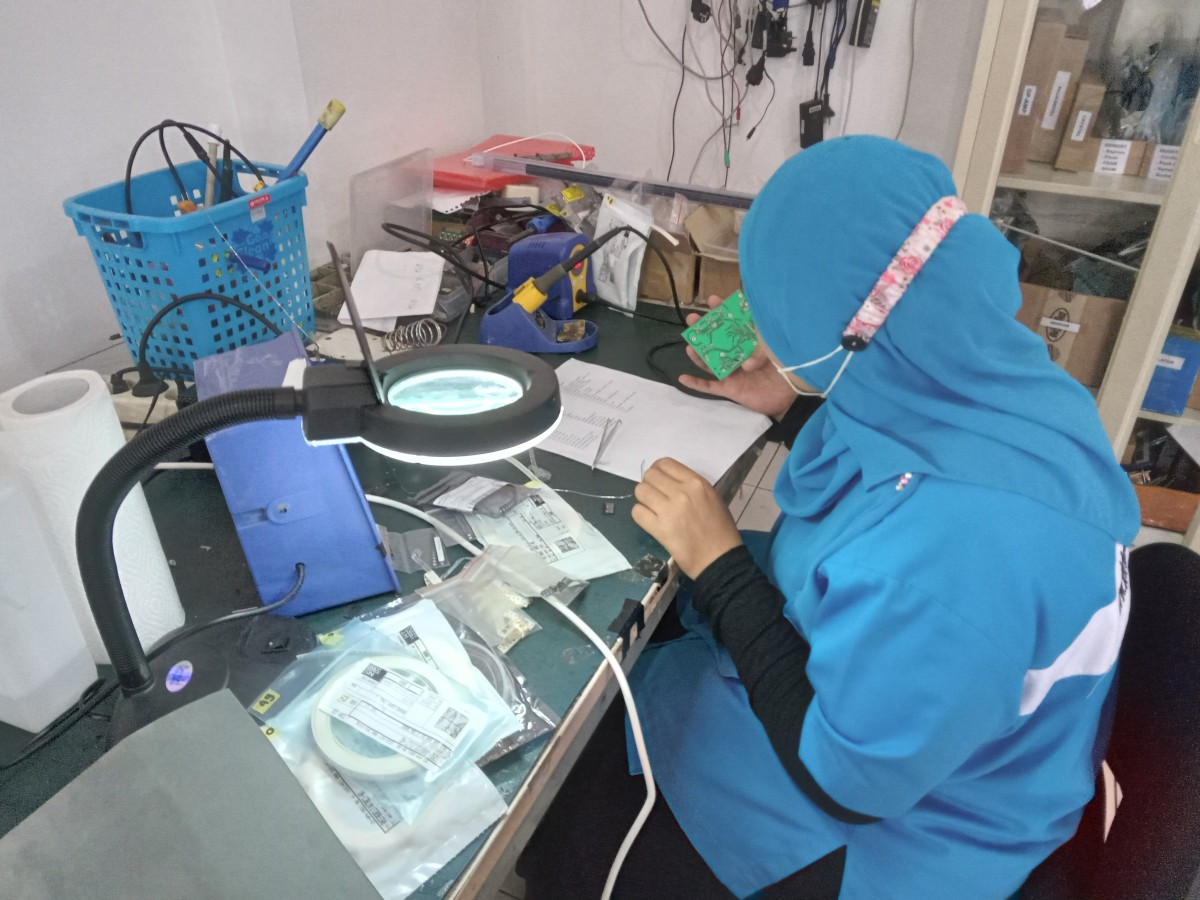
\includegraphics[width=200pt]{images/assembly_manual}
			\end{center}
		\end{exampleblock}
	\end{frame}

	\section{Review Class-D Audio DAC}
	
	\begin{frame}
		\subsection{Tujuan}
		\begin{exampleblock}{Review Class-D AudioDAC}
			Audio Digital to Analog chip yang digunakan adalah seri MAX98357A yang merupakan audio amplifier kelas D.
			Ditemukan frekuensi lebih dari satu frekuensi setiap proses \textit{tone generation} yang muncul saat diuji dengan Audio Capture.
			Perangkat Audio Capture yang digunakan adalah MiniDSP E.A.R.S melalui software DSSF3 buatan Yoshimasha.
		\end{exampleblock}
	
		\begin{exampleblock}{MiniDSP EARS}
			\begin{center}
				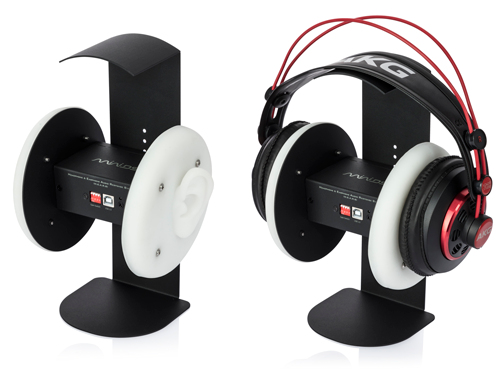
\includegraphics[width=150pt]{images/ears}
			\end{center}
		\end{exampleblock}
	\end{frame}

	\begin{frame}
		\subsection{High Frequency Noise}
		\begin{exampleblock}{Perbandingan penuh dan teratenuasi}
			\begin{center}
				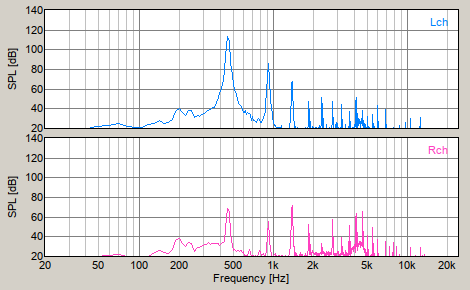
\includegraphics[width=200pt]{images/notattenuated}
				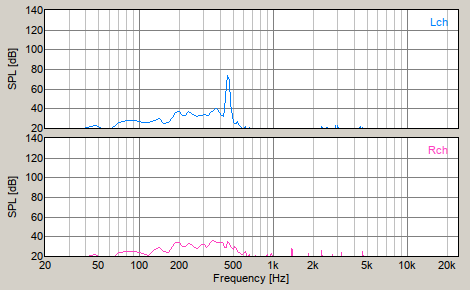
\includegraphics[width=200pt]{images/attenuated}
			\end{center}
		\end{exampleblock}
	\end{frame}
	
	\begin{frame}[fragile]
		\subsection{Signal Generation Code}
		\begin{exampleblock}{Perbaikan Programming}
			Dilakukan perbaikan \textit{programming} terkait metode \textit{tone generation}
		\end{exampleblock}
	
		\begin{exampleblock}{Diff code}
			\begin{minted}[frame=lines,framesep=2mm,baselinestretch=1.2,bgcolor=LightGray,fontsize=\tiny,linenos]{diff}
-static uint16_t i2s_tx_buf[TOTAL_BUFF_SIZE];
+int16_t i2s_tx_buf[TOTAL_BUFF_SIZE];

uint16_t i;
uint16_t buffsize;
double ysin;

for(i=0;i<buffsize;i++){
	ysin = DEFAULT_ATTEN*ampl*32767*sin(2*3.141592653589793*((double)i/(double)buffsize));
	
-	if(ysin >= 0){
-		i2s_tx_buf[i]=ysin;
-	}
-	if(ysin < 0){
-		i2s_tx_buf[i]=ysin+65535;
-	}
+ 	i2s_tx_buf[i] = ysin;
}
			\end{minted}
		\end{exampleblock}
	\end{frame}
	
	\subsection{Clipping Limitation}
	
	\subsection{Compare to Signal Generator}
	
	\section {Review Sementara Desain P3}
	
	\section{Upgrade Packaging P2}
\end{document}
